
%%%%%%%%%%%%%%%%%%%%%
%  Блок "Утверждаю"
%%%%%%%%%%%%%%%%%%%%%
\noindent\parbox[l][7cm]{7cm}
{
	 \begin{center}
 \small\textbf{ООО "ЮЖНО-РЕГИОНАЛЬНАЯ ЭКСПЕРТНАЯ ГРУППА"} \centerline{   }
\scriptsize {ИНН 2311213020 КПП 231101001
	 ОГРН 1162375014560}\\
\footnotesize{350072, Россия, Краснодарский край, Ростовское шоссе, 14/2, оф. 67, (861)2-388-399, моб.: 8-918-451-66-11 }
		\end{center}

\hbox to 6cm{\dotfill А.~В.~Мраморнов}}\hfill\parbox[l][7cm]{6cm}
{

 \begin{center}
	\small\textbf{ООО "ЮЖНО-РЕГИОНАЛЬНАЯ ЭКСПЕРТНАЯ ГРУППА"} \centerline{   }
	\scriptsize {ИНН 2311213020 КПП 231101001
		ОГРН 1162375014560}\\
	\footnotesize{350072, Россия, Краснодарский край, Ростовское шоссе, 14/2, оф. 67, (861)2-388-399, моб.: 8-918-451-66-11 }
\end{center}
\hbox to 6cm{\dotfill А.~В.~Мраморнов}}\hfill\parbox[l][7cm]{6cm}


%%%%%%%%%%%%%%%%%%%%%%%%%
% Бок из двух колонок
%%%%%%%%%%%%%%%%%%%%%%%%%
\noindent\parbox[l][5cm]{6cm}{ДФAAL~DKDKDnnnnn-nnnnnnnnnn   mmmmmmmmmmm   mmmmmmmm mmmmmmmmmm mmmmmmmmmmm mmmmmmmm mmmmmmm mmmmmmmmmmm mmmKK FFHHH hdhdhdhhd ррвррввррврврр } \hfill\parbox[l][5cm]{11cm}{ДФAAL DKDKDnnnnnnnnnnnnnnn   mmmmmmmmmmm   mmmmmmmm mmmmmmmmmm mmmmmmmmmmm mmmmmmmm mmmmmmm mmmmmmmmmmm mmmKK FFHHH hdhdhdhhd ррвррввррврврр }

%%%%%%%%%%%%%%%%%%%%%%%%%%%%%%%%
% Пример выделения абзаца с отступом слева
%%%%%%%%%%%%%%%%%%%%%%%%%%%%%%%
\begin{flushleft} 
	\hbox{% 
		\vrule\hspace{.8em}\parbox{1\textwidth}% 
		{Иногда используется следующий способ выделения текста: абзац набирается с некоторым отступом от левого поля, а слева от него, вровень с левым полем, печатается вертикальная линейка.}} 
\end{flushleft}



%%%%%%%%%%%%%%%%%%%  Водяной знак    %%пакет \usepackage{draftwatermark}
%%%%%%%%%%%%%%%%%%%%%%%%%%%

\SetWatermarkLightness{1} % прозрачность
\SetWatermarkText{} % Текст водяного знака
\SetWatermarkScale{0.8}  %масштаб


%%%%%%%%%%%%%%%%%%%%%%%%%%%%%%%%
% Пример два изображения рядом
%%%%%%%%%%%%%%%%%%%%%%%%%%%%%%%
\begin{figure}[h!]\centering
	\parbox[t]{0.49\textwidth}
	{\centering
		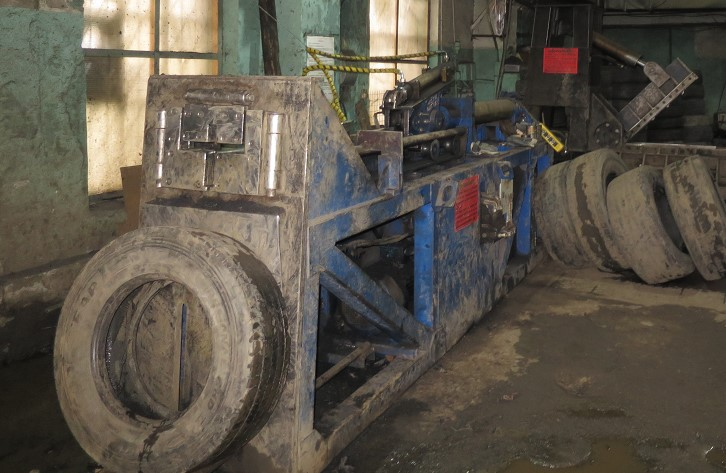
\includegraphics[width=.49\textwidth]{images/1}
		\caption{\footnotesize {Этапы реконструкции ДТП}}
		\label{ris:images/1}}
	\hfil \hfil%раздвигаем боксы по горизонтали 
	\parbox[t]{0.49\textwidth}
	{\centering
		\includegraphics[width=.49\textwidth]{images/39}
		\caption{\footnotesize {Этапы реконструкции ДТП}}
		\label{ris:images/39}}
\end{figure}


%%%%%%%%%%%%%%%%%%%%%%%%%%%%%%%%
% Пример изображения рядом подпись к изображению  и само изображение
%%%%%%%%%%%%%%%%%%%%%%%%%%%%%%%

\begin{SCfigure}
	\centering {\footnotesize \caption{Схематичное изображение перераспределения веса автомобиля при торможении  под действием силы $ \vec{F_t}  $ }} 
	\includegraphics[width = 0.6 \textwidth]{example-image}
	\label{ris:images/tormoz}
\end{SCfigure}


%%%%% Текст рядом с изображением


\noindent\begin{minipage}{0.4\linewidth}
    {Величина усилия разрыва болтового соединения известна,
        тогда по правилу отношения плечей приложенных сил: 
        \begin{equation}\label{схемаразрыва}
        \frac{\vec{F_1}}{\vec{F_2}} = \frac{l_2}{l_1}  
        \end{equation}
        $ l_2/l_1 = 470/155 \approx 1/3 $, 
        
        получаем, что для создания усилия разрыва в точке "А", необходимо к точке "В" приложить усилие, равное $\vec{ F_2} = \vec{F_1}/3 = 6 485/3 \approx 2 161 kg $
    }
\end{minipage}
\hfill
\begin{minipage}{0.6\linewidth}
    \begin{center}
        \includegraphics[width=0.9\linewidth]{example-image}
    \end{center}
    \captionof{figure}{Эскиз зуба с расположением разрывных болтов}
\end{minipage}

%%%%%%%%%%%%%%%%%%%%%%%%%%%%%%%%%%%%
%% Два рядом с одной общей подписью 
%%%%%%%%%%%%%%%%%%%%%%%%%%%%%%%%%%%%

\begin{figure}[]
	\begin{minipage}{0.49\textwidth}
		\includegraphics[width=\linewidth]{example-image}
		\subcaption{This is a subfigure}
	\end{minipage}
	\hfill
	\begin{minipage}{0.49\textwidth}
		\includegraphics[width=\linewidth]{example-image}
		\subcaption{This is another subfigure}
	\end{minipage}
	
	\caption{This is a caption for the entire figure}
	\label{fig:twosubs}
\end{figure}



%%%%%%%%%%%%%%%%%%%%%%%%%%%%%%%%%
%  Таблица работ
%%%%%%%%%%%%%%%%%%%%%%%%%%%%%%%%%

\begin{center}
	\begin{tabulary}{\textwidth}{LCL}
		\hline 
		\textbf{Наименование детали}      &   & \textbf{Ремонтное воздействие}\\
		\hline Турбина левая              &   &    Заменить\\
		Блок ДВС                          &   &    Отремонтировать гильзованием, заменой колец и прокладок \\
	\end{tabulary}  
\end{center}


%%%%%%%%%%%%%%%%%%%%%%%%%%%%%%%%%%%%%
% История автомобиля
%%%%%%%%%%%%%%%%%%%%%%%%%%%%%%%%%%%%%
{\small 
	\begin{longtable}{|p{16mm}|p{12mm}|p{29mm}|p{50mm}|p{41mm}|}
		\caption[]{\footnotesize {\textbf{История ремонта и сервисного обслуживания по дате и пробегу}}} \label{tab:hist}\\
		\hline
		%\rowcolor[HTML]{C0C0C0} 
		% Заголовки столбцов
		\textbf{Дата} &\textbf{Пробег, км} &\textbf{№\,Заказ-наряда, накладной}& \textbf{Вид работы}& \textbf{Примечание} \\ \hline \endhead % повторение заголовка 
		% Строки
		22.22.2019 &33\,000  & № 480279303-1 от 03.09.2019& Панель задка  & Замена, окраска \\ \hline
		%\rowcolor[HTML]{EFEFEF} 
		\Rownum & &n & Боковина задняя левая   & Замена, окраска \\ \hline
		%%% ..............& 
	 % Обнуляем счетчик строк для следующей таблицы
	\end{longtable}}
\setcounter{rownum}{0} %сброс счетчика строк в таблице

%%%%%%%%%%%%%%%%%%%%%%%%%%%%%%%%%%%%%%
% Длинная таблица
%%%%%%%%%%%%%%%%%%%%%%%%%%%%%%%%%%%%%%
\begin{longtable}{|p{1cm}|p{11cm}|p{3cm}|}
	\caption[]{\footnotesize {Ремонтные воздействия}} \label{tab:4}\\ 
	\hline
	\rowcolor[HTML]{C0C0C0} 

	\text{N/N} & Наименование запчасти (материала) & Ремонтное воздействие  \\ \hline \endhead % повторение заголовка 
	\Rownum  & Панель задка  & Замена, окраска \\ \hline
	\rowcolor[HTML]{EFEFEF} 
\Rownum  & Боковина задняя левая   & Замена, окраска \\ \hline
	%%% ..............
\end{longtable}

%%%%%%%%%%%%%%%%%%%%%%%%%%%%%%%%%%%%%%%%%%%%%%%
% Таблица аналогов
%%%%%%%%%%%%%%%%%%%%%%%%%%%%%%%%%%%%%%%%%%%%%%%%
\begin{longtable}{|p{5mm}|p{85mm}|p{60mm}|}
	\caption[]{\footnotesize {Описание ТС, идентичных оцениваему}} \label{tab:5}\\ 
	\hline
	\rowcolor[HTML]{C0C0C0} 
	\bf	\text{n/n} &\bf  Описание аналога & \bf URL-адрес преложения  \\ \hline \endhead
	\toprule \centering
	\Rownum  &\includegraphics[width=0.99\linewidth]{A_1} &\noindent {\scriptsize\ https://krasnodar.drom.ru/mazda/mazda6/34943451} \\ \hline 	\centering
	%	\rowcolor[HTML]{EFEFEF} 
	\Rownum  &\includegraphics[width=0.99\linewidth]{A_2} & {\noindent \centering  \scriptsize\ https://krasnodar.drom.ru/mazda/mazda6/34943451} \\ \hline 	\centering
	
\end{longtable}

%%%%%%%%%%%%%%%%%%%%%%%%%%%%%%%%%%%%%%%%
% Таблица длинная по типу таблицы годных остатков
%%%%%%%%%%%%%%%%%%%%%%%%%%%%%%%%%%%%%%%

\begin{longtable}{|p{9cm}|p{4cm}|p{2cm}|}
	\caption[]{\footnotesize {Таблица расчета $ C_i $ }}
	\label{tab:7}\\
	\hline
	Наименование агрегата, узла, детали & \%-ное соотношение (вес)  & Годные, \% \\
	\hline \endhead
	Кузовные детали, экстерьер, интерьер, в т.ч.: & 50 (45 \textless{}1\textgreater{}) & 0 \\
	Передняя часть: & 14 &  \\
	Капот & 1.9 & 1,9 \\
	Крыло переднее (за 1 шт.) & 0.8 & 0,8 \\

	Прочее & 3/8 \textless{}1\textgreater{}/1 \textless{}2\textgreater /6 \textless{}3\textgreater{} & 4 \\
	\hline
	\textbf{ИТОГО,} \%: &  & \textbf{83,8}  \\
	\hline	
\end{longtable}
%%%%%%%%%%%%%%%%%%%%%%%%%%%%%%%%%%%%%%%%%
%%% Таблица с объединением строк 
%%%%%%%%%%%%%%%%%%%%%%%%%%%%%%%%%%%%%%%%%
\begin{table}[H]
	\caption{\label{tab:bolts} Нестандартные болты для левой резьбы.}
	\begin{center}
		\begin{tabular}{|c|c|c|}
			\hline
			\multirow{3}{*}{Размеры нестандартных болтов} & \multicolumn{2}{c|}{Диаметр} \\
			\cline{2-3}
			& Норма & Разброс \\
			\cline{2-3}
			& 10 мм & 1 мм \\
			\hline
		\end{tabular}
	\end{center}
\end{table}
%%%%%%%%%%%%%%%%%%%%%%%%%%%%%%%%%%%%%%%%%
%% Таблица с объединение строк и столбцов
%%%%%%%%%%%%%%%%%%%%%%%%%%%%%%%%%%%%%%%%%%

\begin{table}[ph]
	\centering
	\begin{tabular}{c|c|c|c|c}
		\hline
		\multirow{2}{*}{Raaa (k)} & \multicolumn{4}{c}{C ()} \\
		\hhline{~----}
		& 3.3 & 2.5 & 1 & 0.5 \\
		\hline
		\multirow{2}{*}{Raaa (k)} & \multicolumn{2}{c|}{\multirow{2}{*}{this}} & 0.5 & 0.6\\
		\hhline{~~~--}            & \multicolumn{2}{c|}{}                      & 0.7 & 1.2 \\
		\hline
	\end{tabular}
	\caption{R, C ripple size}
	\label{T:peak}
\end{table}

%%%%%%%%%%%%%%%%%%%%%%%%%%%%%%%%%%%%%%%%%%
%%%%  Таблица повреждений автомобиля
%%%%%%%%%%%%%%%%%%%%%%%%%%%%%%%%%%%%%%%%%%
\begin{longtable}{|M{125mm}|M{30mm}|}
	\caption[]{\footnotesize {Повреждения автомобиля, установленные при его осмотре}} \label{tab:5}\\ 
	\hline
\bf {\small Наименование поврежденной детали с описанием повреждения} & \bf {\small Изображение} \\ \hline \endhead
	%
% {\small    } & \imt{fp1} \\ \hline  % Фото повреждений
	%
{\small Дверь передняя левая -  деформация в труднодоступном месте на площади 6дм2}&  \imt{example-image}\\ \hline 
% {\small    } & \imt{fp1} \\ \hline  % Фото повреждений
% {\small    } & \imt{fp1} \\ \hline  % Фото повреждений
% {\small    } & \imt{fp1} \\ \hline  % Фото повреждений
% {\small    } & \imt{fp1} \\ \hline  % Фото повреждений
% {\small    } & \imt{fp1} \\ \hline  % Фото повреждений
% {\small    } & \imt{fp1} \\ \hline  % Фото повреждений
% {\small    } & \imt{fp1} \\ \hline  % Фото повреждений

\end{longtable}


%%%%%%%%%%%%%%%%%%%%%%%%%%%%%%%%%%%%%%%%%%%%%
%%%%  Таблица ремонтных воздействий
%%%%%%%%%%%%%%%%%%%%%%%%%%%%%%%%%%%%%%%%%%%%%
\begin{longtable}{|p{1cm}|p{11cm}|p{3cm}|}
	\caption[]{\footnotesize {Ремонтные воздействия по акту осмотра № 006/06/19 от \, \osm \, ИП Яковлева С.В.}} \label{tab:4}\\ 
	\hline
	\rowcolor[HTML]{C0C0C0} 
	%	\multicolumn{1}{|c|}
	%	{\cellcolor[HTML]{C0C0C0}N/N} & Наименование запчасти (материала) & Ремонтное воздействие 
	%	
	\text{N/N} & Наименование запчасти (материала) & Ремонтное воздействие  \\ \hline \endhead
	\Rownum  & Панель задка  & Замена, окраска \\ \hline
	\rowcolor[HTML]{EFEFEF} 
	\Rownum  & Боковина задняя левая   & Замена, окраска \\ \hline
	\Rownum  & Боковина задняя правая  & Замена, окраска  \\ \hline
	
\end{longtable}\setcounter{rownum}{0}

%%%%%%%%%%%%  Загрузка данных из csv
                         %%%%%%%%%   CSV    %%%%%%%%%%%%%
\csvautobooklongtable[separator=comma]{test.csv} % semicolon- ;  comma- , pipe- | tab- 	
%%%%%%%%%%%%%%%%%%%%%%%%%%%%%%%%%%%%%%%%%%%%%%%%%%%


%%%%%%%%%%%%%%%%%%%%%% 
%%%  Изображение заданного рамера
%%%%%%%%%%%%%%%%%%%

\includegraphics*[width=5.54in, height=1.66in, keepaspectratio=false]{example-image}
%

%%%%%%%%%%%%%%%%%%%%%%%%%%%%%%%%%%%%%   Сноски %%%%%%%
 \footnote{текст сноски}

%%%%%%%%%%%%%%%%%%%%%%
% \usepackage{array} is required
\begin{tabular}{|>{\raggedright\arraybackslash}p{30mm}|>{\raggedright\arraybackslash}p{95mm}|>{\raggedright\arraybackslash}p{30mm}|}
	\hline 
	&  &  \\ 
	\hline 
	&  &  \\ 
	\hline 
	&  &  \\ 
	\hline 
\end{tabular} 
% \usepackage{array} is required
\begin{tabular}{|>{\raggedleft\arraybackslash}p{3cm}|>{\raggedleft\arraybackslash}p{3cm}|>{\raggedleft\arraybackslash}p{3cm}|}
	\hline 
	&  &  \\ 
	\hline 
	&  &  \\ 
	\hline 
\end{tabular} 
% \usepackage{array} is required
\begin{tabular}{|>{\raggedright\arraybackslash}p{3cm}|>{\centering\arraybackslash}p{%<3cm%>}|>{\centering\arraybackslash}p{%<3cm%>}|}
			\hline 
			&  &  \\ 
			\hline 
			&  &  \\ 
			\hline 
		\end{tabular} 
		
		
%%%%%%%%%%%%%%% ПРОСТАЯ ТАБЛИЦА ПОВРЕЖДЕНИЙ

{\small \begin{table}[]
\begin{longtable}{@{}ll@{}}
	\caption[]{\footnotesize {\textbf{Описание повреждений деталей}}} \label{tab:4}\\ 
		\toprule
	\textbf{	Наименование детали       }               &\textbf{ Описание повреждений}                         \\ \midrule
		Решетка бампера переднего средняя        & разбита                                      \\
		Решетка бампера левая                    & оборваны, деформированы крепежные кронштейны \\
		%.................................
		Заднее правое крыло                      & несложная деформация, повреждение ЛКП        \\ \bottomrule
	\end{longtable}
\end{table}}

%%%%%%%%%%%%%%%%% ПРОСТАЯ ТАБЛИЦА РЕМОНТНЫХ ВОЗДЕЙСТВИЙ

{\small \begin{table}
	\begin{longtable}{@{}ll@{}}
	\caption[]{\footnotesize {\textbf{Назначенные ремонтные воздействия}}} \label{tab:2}\\ 
	\toprule
\textbf{Наименование детали}                      & \textbf{Ремонтные воздействия}\\ \midrule
Решетка бампера переднего средняя        & заменить             \\
%......................
Заднее правое крыло                      & ремонт 3 ч, окрасить \\ \bottomrule
\end{longtable}

\end{table}}


%%%%%%%%%%%%%%%%%%%%%%%%%%%%%%%%%%%
%%%
%%% ТАБЛИЦА  ДЛИННАЯ ТОНОВАЯ РАЗМЕТКА
%%%%%%%%%%%%%%%%%%%%%%%%%%%%%%%%%%%
 \begin{table}[H]
 	\centering
  	\caption{{\footnotesize Запчасти и материалы к заказ-наряду № Ш000011955 от 10.08.2017}}
 	\label{tab:4}
 	\begin{tabular}{|l|ll|l|l|}
 		\hline
 		\rowcolor[HTML]{C0C0C0} 
 		\multicolumn{1}{|c|}{\cellcolor[HTML]{C0C0C0}N кат} & Наименование запчасти (материала) & & Цена за шт. & Всего цена, руб \\ \hline
		7109113821    & Хомут пластиковый самозатяжной  & & 5      & 50      \\ \hline
	    \rowcolor[HTML]{EFEFEF} 
		0411151042    & Ремкомплект ДВС 1VDFTV (1 шт.)      & & 16000     & 16000    \\ \hline
		1111551030С0    & Прогкладка ГБЦ правая  (1 шт.)    & & 3250     & 3250      \\ \hline
		\rowcolor[HTML]{EFEFEF} 
		1111651030С0    & Прокладка ГБЦ левая (1 шт.) & & 3250     & 3250      \\ \hline
		131010W011B0    & Поршень левый (4 цил)      & & 4900     & 19600      \\ \hline
		\rowcolor[HTML]{EFEFEF} 
		131010W021B0   & Поршень правый (4 цил.)  & & 5000     & 20000      \\ \hline
		1301151040    & Кольца поршневые комплект (8цил)      & & 38     & 49000      \\ \hline
%%%  ........................
			\rowcolor[HTML]{EFEFEF} 
 		103223   & Масло трансмиссионное Multi ATF (1.3 л)     & & 750   & 975      \\ \hline
 	%	17   & Клапан (16 шт.)       & 1150     & 18400      \\ \hline& 
 		\end{tabular}
\end{table}